\documentclass{cmspaper}
\begin{document}

\section{Cut Optimization} \label{sec:cutOptimization}

The optimal cut values for the selection criteria are chosen in order to minimize the estimate of the upper limit on the signal cross section based on the Bayesian approach described in section XX.

The results for the optimal cut values for the object $p_T$ are consistently the lowest value in the scanned range.  However, an increase in the cut value of the object $p_T$ is seen to have only a small effect on the significance of the signal.  Higher than optimal cut values for the $p_T$ are chosen in order to reduce the effect of initial and final state radiation and contamination of the object collections by misidentified objects.  

A hard cut on the ST of the event shows the strongest discriminating power of the selection criteria.  This quantity is shown in figure \ref{fig:optimization} a) for both a 400 GeV signal sample and for the dominant background.  The optimal cut value on ST scales with the mass hypothesis for the leptoquark.  Figure \ref{fig:optimization} b) shows the variation on the upper limit of the cross section as a function of varying ST cut on a 400 GeV leptoquark sample with standard model background estimates for $100 pb_{-1}$.

\begin{figure}[htbp]
  \begin{center}
    \begin{tabular}{cc}
      \resizebox{7.5cm}{!}{a)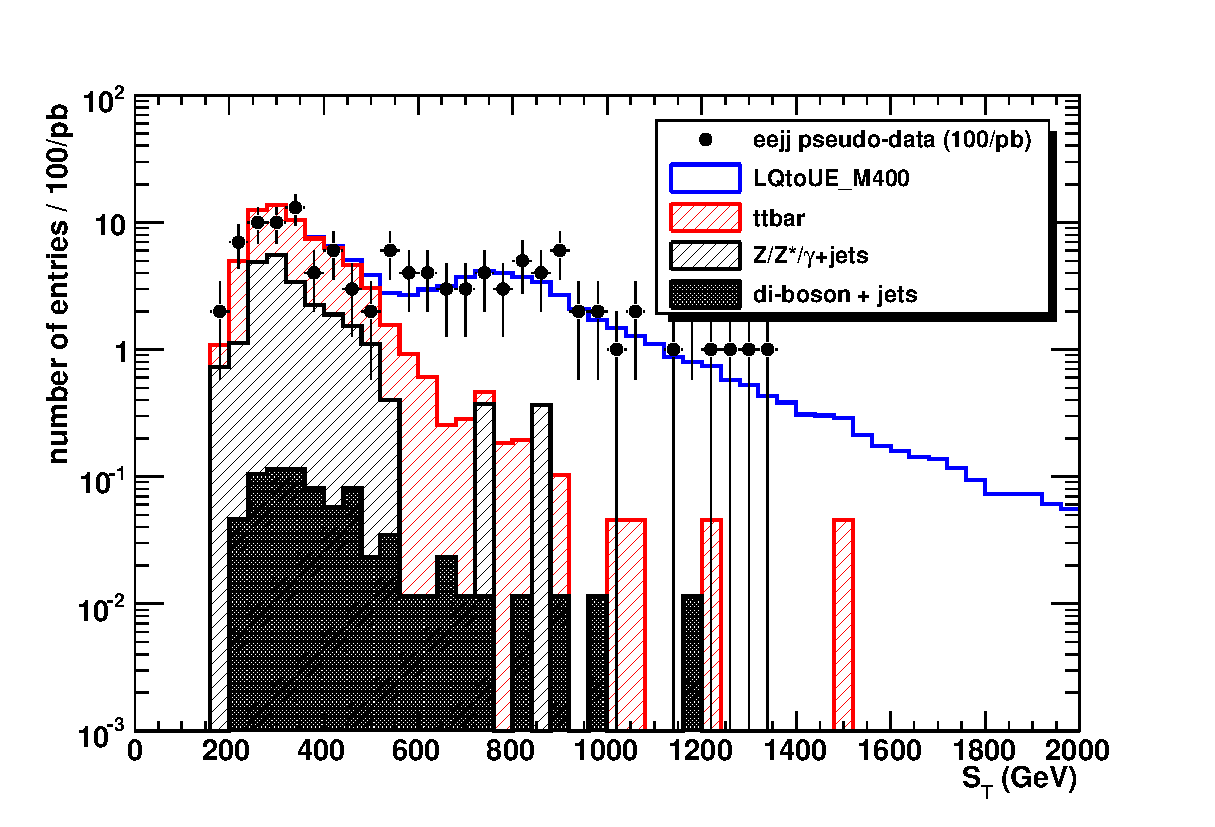
\includegraphics{plots/ST_eejj_LQ400_100pb.eps}} &
      \resizebox{7.5cm}{!}{b)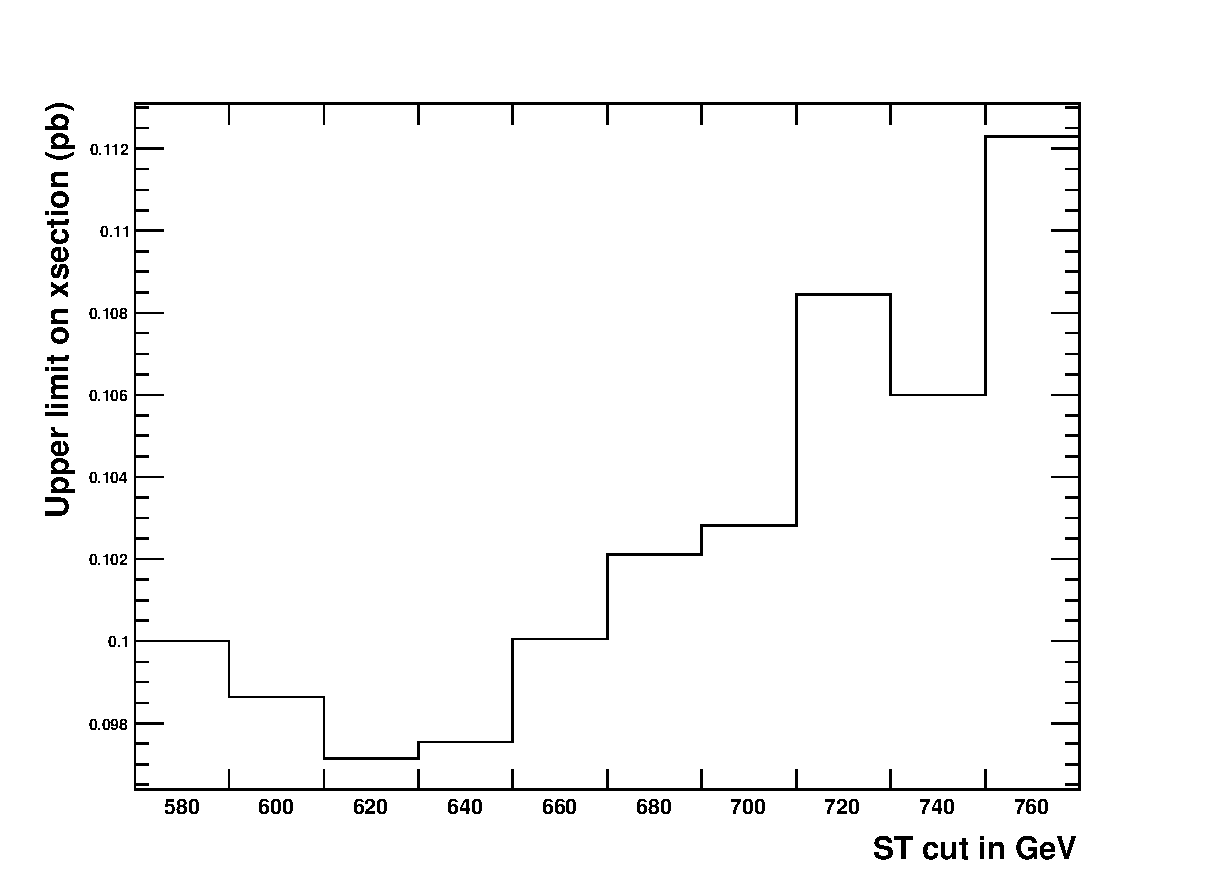
\includegraphics{plots/xSecLimit_M400.eps}} \\
    \end{tabular}
    \caption{\small \sl a) Distribution of ST variable for 400 GeV leptoquark signal and standard model background rescaled to 100 $pb^{-1}$, along with pseudo data for 100 $pb^{-1}$, b) Upper limit on the signal cross section for a range of ST cuts }
    \label{fig:optimization}
  \end{center}
\end{figure}



\end{document}
